\chapter{Results}
\label{cha:results}
In the next two sections I will illustrate and discuss the results of the main two abstract components of my project: the \textit{Symptom Identifier} and the \textit{Symptom Classifier}.

\section{Evaluation of the Symptom Identifier}
\label{sec:eval_symptom_identifier}
In order to evaluate the Symptom Identifier, I manually classified the tokens for predictions of each sentence in four classes (just to recall, tokens for predictions are the outcome of the Symptom Identifier):
\begin{itemize}
  \item \texttt{correct} tokens. These are tokens that contain an intelligible symptom that is also present in the patient's sentence;
  \item \texttt{redundant} tokens. These tokens are correct but redundant (there is another token that has the same meaning);
  \item \texttt{non sense} tokens. These tokens are simply not intelligible;
  \item \texttt{wrong} tokens. These tokens are deceptive because they contain an intelligible symptom but they are not present in patient's sentence.
\end{itemize}

Finally, for each sentence, I noted also the number of symptoms present in the sentence but not in the tokens (\texttt{missing}).

In order to choose the best model for future evaluations, I designed a score metric that summarizes the performance of this component. Just for a matter of clarity, ``\texttt{\#C}'' means ``total number of predictions belonging to the class \texttt{C}'':
\begin{equation}
score = \texttt{\#correct} + 0 \cdot \texttt{\#redundant} - \texttt{\#non sense} - \texttt{\#wrong} - \texttt{\#missing}
\end{equation}

The reader may wonder why is a \texttt{non sense} token so penalized. The reason is that this type of token is detrimental as much as a wrong one because it leads to a random prediction. Instead, a redundant token is neutral because it probably leads to a duplicated, but correct, prediction.

Here is an overview of the obtained results:

\definecolor{green}{rgb}{0.8,0.9,0.8}
\definecolor{lightgreen}{rgb}{0.89, 0.94, 0.89}
\definecolor{red}{rgb}{1,0.89,0.89}

\begin{center}
 \begin{tabular}{| c | c | c | c |} 
 \hline
 \# of & BERT & R-NET \\ [0.5ex] 
 \hline\hline
 \rowcolor{green}
 \texttt{correct} & 423 & 427 \\ 
 \hline
 \rowcolor{lightgreen}
 \texttt{redundant} & 275 & 195 \\
 \hline
 \rowcolor{red}
 \texttt{non sense} & 122 & 247 \\
 \hline
 \rowcolor{red}
 \texttt{wrong} & 8 & 14 \\
 \hline
 \rowcolor{red}
 \texttt{missing} & 61 & 74 \\
 \hline
 \textbf{score} & \textbf{232} & \textbf{92} \\ 
 \hline
\end{tabular}
\end{center}

The results, and, in particular, the score measure, suggest that BERT is consistently better for this task. For this reason I used its outcome as input for the evaluation of the Symptom Classifier.

However, some more measures could help to understand the real performances of the two models. Numerically, using BERT, the percentage of correct and redundant TFPs is $84.8 \%$ ($\frac{\texttt{\#correct} + \texttt{\#redundant}}{\texttt{\#TFP}}$); against the $70.4 \%$ when using R-NET. If we consider only the correct TFPs ($\frac{\texttt{\#correct}}{\texttt{\#TFP}}$), the percentage decreases to $52.6 \%$ (against the $48.4 \%$ when using R-NET). This component, always using BERT, can identify the $88.0 \%$ of symptoms present in sentences ($\frac{\texttt{\#correct}}{\texttt{\#correct} + \texttt{\#missings}}$). The percentage using R-NET is more or less the same ($87.5 \%$). The following table summarizes these results.

\newcolumntype{C}{ >{\centering\arraybackslash} m{4cm} }
\newcolumntype{D}{ >{\centering\arraybackslash} m{2cm} }
\begin{center}
 \begin{tabular}{| C | D | D |}
 \hline
 measures & BERT & R-NET \\ [1ex] 
 \hline\hline
 \texttt{$\frac{\texttt{\#correct} + \texttt{\#redundant}}{\texttt{\#TFP}}$} & 84.8 \% & 70.4 \% \\[1ex]
 \hline
 \texttt{$\frac{\texttt{\#correct}}{\texttt{\#TFP}}$} & 52.6 \% & 48.4 \% \\[1ex]
 \hline
 \texttt{$\frac{\texttt{\#correct}}{\texttt{\#correct} + \texttt{\#missings}}$} & 88.0 \% & 87.5 \% \\[1ex]
 \hline
\end{tabular}
\end{center}

\section{Evaluation of the Symptom Classifier}
\label{sec:evalsymptomclassifier}
\subsection{Definitions and notation}

The expression ``$\texttt{real cuis}_{i}$'' refers to the list of real symptom CUIs of the i-th sentence. Analogously, the expression ``$\texttt{predicted cuis}_{i}$'' refers to the list of predicted CUIs of the i-th sentence.

The symbol ``\texttt{\#}'' in front of a list identifier indicates its length.

\subsubsection{Types of predictions}
The predictions are based on the \textit{tokens for prediction} and can be classified as:
\begin{itemize}
  \item \texttt{correct}, if the prediction is located in a subtree rooted in any of the \texttt{real cuis}. Correct predictions can be of two types:
    \begin{itemize}
      \item \textit{redundant} (\texttt{R}). When a prediction is mapped to a subtree, the subtree is marked as associated with that prediction. Then, if another prediction of the same sentence stays in that subtree, it is classified as redundant;
      \item \textit{non-redundant} (\texttt{NR}), if the prediction stays in a unmarked subtree;
    \end{itemize}
  \item \texttt{wrong}, if the prediction is not located in any of the subtrees.
\end{itemize}

These terms are also contextual to the sentence: this means that they can be indexed as well. To give an example, $\texttt{\#correct}_{i}$ represents the number of correct predictions of the i-th sentence.

\subsection{Measures}
This component performs a slight variation of multi-class classification (a class for each symptom present in the tree). The variation stands in the ``pruning'' option (the number of candidate classes decreases) and in the fact that if the predicted CUI and the real one are different (i.e. they are different classes), the prediction could be correct (if the prediction is in the subtree of the real CUI).

Once understood the complex nature of this task, is not surprising that, apart from accuracy, there are not any standard measures used to summarize the its results. For example, precision, recall and F1 score suit only for binary classification. This led me to develop my own measures, designed exclusively for this task.

The first measure is \texttt{accuracy} and it represents the fraction of symptoms that were predicted correctly over the total number of symptoms:
\begin{equation}
\texttt{accuracy} = \frac{\sum_{i}{\texttt{\#correct}_{i}^{\texttt{NR}}}}{\sum_{i}{\texttt{\#real cuis}_{i}}}
\end{equation}

The second measure is \texttt{\% of correct predictions} and it is the fraction of the number of correct predictions (redundant and non-redundant) over the total number of predictions. This measure represents the probability, for a prediction, of being correct:
\begin{equation}
\texttt{\% of correct predictions} = \frac{\sum_{i}{\texttt{\#correct}_{i}}}{\sum_{i}{\texttt{\#predicted cuis}_{i}}}
\end{equation}

The following measure, called \texttt{medium attempts}, is computed as the total number of predictions over the total number of actual symptoms present in the sentences. It represents the medium number of attempts that the model does for each symptom a the sentence:
\begin{equation}
\texttt{medium attempts} = \frac{\sum_{i}{\texttt{\#predicted cuis}_{i}}}{\sum_{i}{\texttt{\#real cuis}_{i}}}
\end{equation}

The fourth measure represents the \texttt{missed symptoms}. Even if it is not indispensable because it is complementary to the \texttt{accuracy}, it can be useful to understand the number of missed tokens (and not its percentage):
\begin{equation}
\texttt{missed symptoms} = \sum_{i}{\texttt{\#real cuis}_{i}} - \sum_{i}{\texttt{\#correct}^{\texttt{NR}}_{i}}
\end{equation}

%%%%%%%%%%\newpage
\subsection{Evaluation of different options}
\label{sec:evaluationoptions}
In this subsection I will show and analyze individually every option of the Symptom Classifier. Those are: the embedding type, if using or not the \textit{Body Part Finder}, if using or not the ``pruning'' option, if using or not the \textit{filter for ``unuseful words''} and the \textit{minimum similarity} level.

\subsubsection{Comparing different types of embeddings}

\begin{figure}[h]%[!tbp]
  \centering
  \begin{minipage}[b]{0.4\textwidth}
    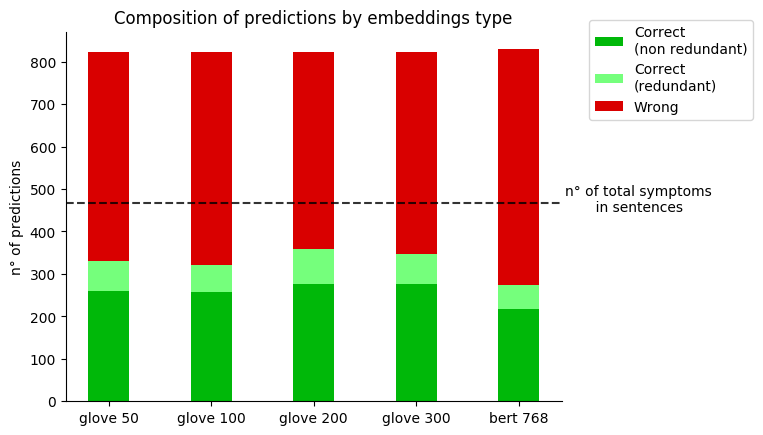
\includegraphics[width=9cm]{graphs/comparison_embeddings_type}
    \caption{Comparing the composition of the predictions across different embedding types.}
  \end{minipage}
  \hfill
  \begin{minipage}[b]{0.4\textwidth}
    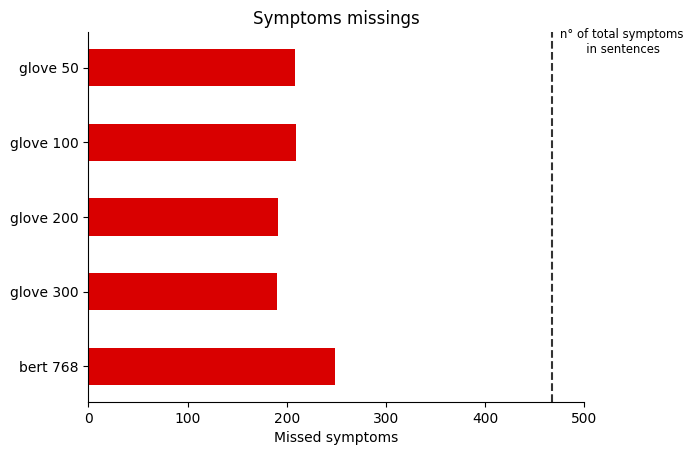
\includegraphics[width=8cm]{graphs/comparison_embeddings_type_missings}
    \caption{Comparing the \texttt{missing symptoms} across different embedding types.}
  \end{minipage}
\end{figure}

\begin{center}
 \begin{tabular}{| c | c | c | c | c | c |} 
 \hline
 \thead{\texttt{embedding}\\\texttt{type}} & \thead{\texttt{accuracy}} & \thead{\texttt{correct}\\\texttt{predictions}} & \thead{\texttt{harmonic}\\\texttt{mean}} & \thead{\texttt{medium}\\\texttt{attempts}} & \thead{\texttt{missed}\\\texttt{symptoms}} \\ [0.5ex] 
 \hline\hline
 \texttt{GloVe 50} & 55.5 \% & 40.1 \% & 46.5 \% & 1.8 & 208 \\ 
 \hline
 \texttt{GloVe 100} & 55.2 \% & 39.1 \% & 45.8 \% & 1.8 & 209 \\
 \hline
 \texttt{GloVe 200} & 59.1 \% & 43.7 \% & 50.2 \% & 1.8 & 191 \\
 \hline
 \texttt{GloVe 300} & 59.3 \% & 42.2 \% & 49.3 \% & 1.8 & 190 \\
 \hline
 \texttt{BERT emb.} & 46.7 \% & 32.9 \% & 38.6 \% & 1.8 & 249 \\
 \hline
\end{tabular}
\end{center}

%%%%%%%%%%%%%%%%%%%%%%%%%%% discuss data

During this test I compared different types of embeddings. As we can see in the table, the performances of \texttt{GloVe 50} and \texttt{GloVe 100} are very similar (we can simply look at the harmonic mean between accuracy and correct predictions because the medium attempts rest the same). However, \texttt{GloVe 200} introduced an improvement compared to \texttt{GloVe 100} (+ 3.9 \% of accuracy and + 4.6 \% of correct predictions ). This trend is also confirmed by \texttt{GloVe 300} (+ 4.1 \% of accuracy and + 3.1 \% of correct predictions). Looking at these results, I choose \texttt{GloVe 200} as the embedding type used for the tests that I will explain in the next sections.

The \texttt{medium attempts} are all equal because the options that cause a decrease of the number of predictions are not enabled: the Body Part Finder cause an increase of them and using zero level of minimum similarity does not affect the number of predictions.

BERT embeddings do not perform as good as GloVe embeddings. This because I extracted the embeddings from a non-finetuned BERT, which has not been trained on any medical corpus. Another possible reason for these poor performance is that I tried only one pooling strategy (second-to-last mean of embeddings). Later, I discovered that there are more suitable pooling strategies that could be used, as showed in the referenced post \cite{poolingstrategies}.

%%%%%%%%%%%%%%%%%%%%%%%%%%%
\newpage
\subsubsection{Ablation test for the Body Part Finder}

\begin{figure}[h]%[!tbp]
  \centering
  \begin{minipage}[b]{0.4\textwidth}
    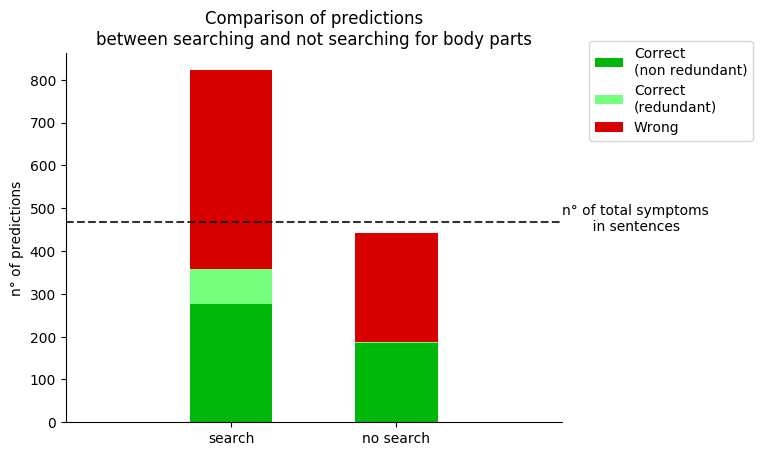
\includegraphics[width=9cm]{graphs/comparison_search_bp}
    \caption{Comparing the composition of the predictions when the Body Part Finder is enabled (\texttt{search}) and when it is not (\texttt{no search}).}
  \end{minipage}
  \hfill
  \begin{minipage}[b]{0.4\textwidth}
    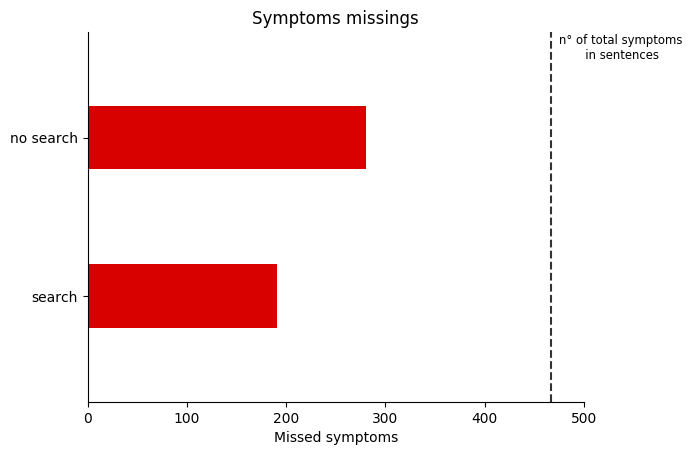
\includegraphics[width=8cm]{graphs/comparison_search_bp_missings}
    \caption{Comparing the \texttt{missing symptoms} when the Body Part Finder is enabled (\texttt{search}) and when it is not (\texttt{no search}).}
  \end{minipage}
\end{figure}

\begin{center}
 \begin{tabular}{| c | c | c | c | c |} 
 \hline
  & \thead{\texttt{accuracy}} & \thead{\texttt{correct}\\\texttt{predictions}} & \thead{\texttt{medium}\\\texttt{attempts}} & \thead{\texttt{missed}\\\texttt{symptoms}} \\ [0.5ex] 
 \hline\hline
 \texttt{search} & 59.1 \% & 43.7 \% & 1.8 & 191 \\
 \hline
 \texttt{no search} & 39.8 \% & 42.2 \% & 0.9 & 281 \\
 \hline
\end{tabular}
\end{center}

%%%%%%%%%%%%%%%%%%%%%%%%%%% discuss data

In Machine Learning an ablation test is a test in which a model is tested without a feature (ablation of the considered feature), and then with it. This is done in order to test the effectiveness of the component.

The introduction of this component led to both pros and cons. The advantage is that there was a large improvement in accuracy (+ 19.3 \%). However, the downside of this percentage lift is that the \texttt{medium attempts} for each symptom in the sentences passed from 0.9 (where there was not enough tokens for prediction in order to cover the \texttt{\#real cuis}) to 1.8 (an excessive number of tokens for predictions).

The percentage of $\texttt{correct}^{\texttt{NR}}$ with respect to the total number of prediction decreased from 41.9 \% (\texttt{no search} for body parts) to 33.5 \% (\texttt{search} for body parts). This was caused by the lift of the number of wrong predictions, that were probably random classifications based on non-sense or wrong tokens for predictions. % For this reason the necessary future work is to limit non-sense tokens.

%%%%%%%%%%%%%%%%%%%%%%%%%%%

\newpage
\subsubsection{Ablation test for the ``pruning'' option}

\begin{figure}[h]%[!tbp]
  \centering
  \begin{minipage}[b]{0.4\textwidth}
    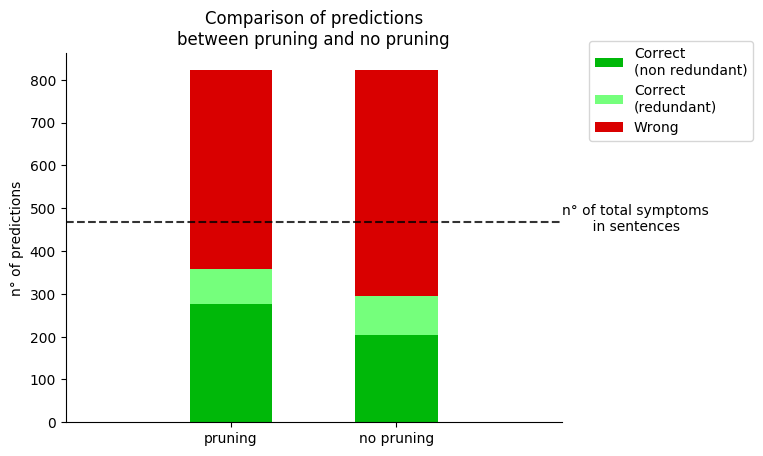
\includegraphics[width=9cm]{graphs/comparison_pruning}
    \caption{Comparing the composition of the predictions when the ``pruning'' option is enabled (\texttt{pruning}) and when it is not (\texttt{no pruning}).}
  \end{minipage}
  \hfill
  \begin{minipage}[b]{0.4\textwidth}
    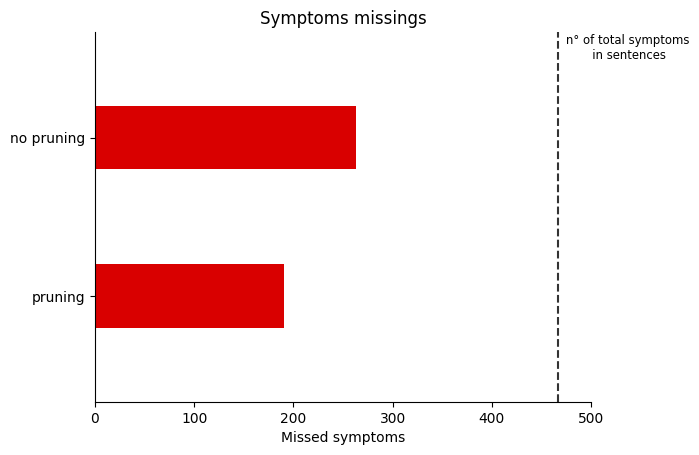
\includegraphics[width=8cm]{graphs/comparison_pruning_missings}
    \caption{Comparing the \texttt{missing symptoms} when the ``pruning'' option is enabled (\texttt{pruning}) and when it is not (\texttt{no pruning}).}
  \end{minipage}
\end{figure}

\begin{center}
 \begin{tabular}{| c | c | c | c | c |} 
 \hline
  & \thead{\texttt{accuracy}} & \thead{\texttt{correct}\\\texttt{predictions}} & \thead{\texttt{medium}\\\texttt{attempts}} & \thead{\texttt{missed}\\\texttt{symptoms}} \\ [0.5ex] 
 \hline\hline
 \texttt{pruning} & 59.1 \% & 43.7 \% & 1.8 & 191 \\
 \hline
 \texttt{no pruning} & 43.7 \% & 36.0 \% & 1.8 & 263 \\
 \hline
\end{tabular}
\end{center}

%%%%%%%%%%%%%%%%%%%%%%%%%%% discuss data

There is little to say about this option: without doubt, it contributes positively to the results. This because with the same number of predictions (the \texttt{medium attempts} score rests the same) it causes an improvement in both \texttt{accuracy} (+ 15.4 \%) and \texttt{correct predictions} (+ 7.7 \%).

%%%%%%%%%%%%%%%%%%%%%%%%%%%

\newpage
\subsubsection{Ablation test for the filter of ``useless words''}
\begin{figure}[h]%[!tbp]
  \centering
  \begin{minipage}[b]{0.4\textwidth}
    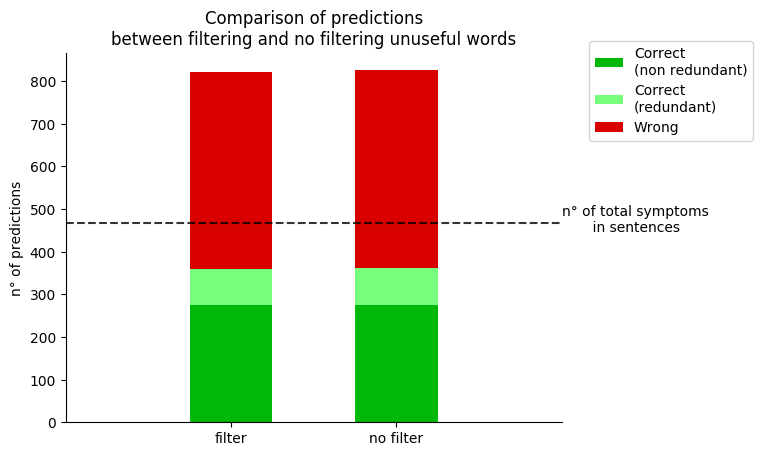
\includegraphics[width=9cm]{graphs/comparison_filtering}
    \caption{Comparing the composition of the predictions when the filtering ``useless words'' option is enabled (\texttt{filter}) and when it is not (\texttt{no filter}).}
  \end{minipage}
  \hfill
  \begin{minipage}[b]{0.4\textwidth}
    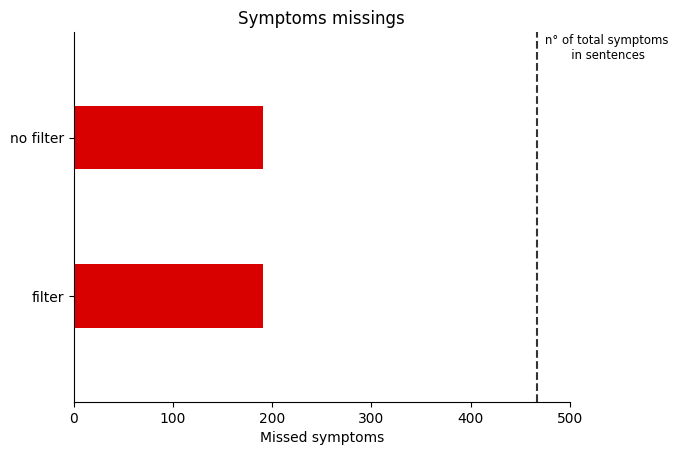
\includegraphics[width=8cm]{graphs/comparison_filtering_missings}
    \caption{Comparing the \texttt{missing symptoms} when the filtering ``useless words'' option is enabled (\texttt{filter}) and when it is not (\texttt{no filter}).}
  \end{minipage}
\end{figure}

\begin{center}
 \begin{tabular}{| c | c | c | c | c |} 
 \hline
  & \thead{\texttt{accuracy}} & \thead{\texttt{correct}\\\texttt{predictions}} & \thead{\texttt{medium}\\\texttt{attempts}} & \thead{\texttt{missed}\\\texttt{symptoms}} \\ [0.5ex] 
 \hline\hline
 \texttt{filter} & 59.1 \% & 43.7 \% & 1.8 & 191 \\
 \hline
 \texttt{no filter} & 59.1 \% & 43.9 \% & 1.8 & 191 \\
 \hline
\end{tabular}
\end{center}

%%%%%%%%%%%%%%%%%%%%%%%%%%% discuss data

This option turned out to be completely ineffective. Personally, I think that the cause is that the Symptom Classifier considers all the possible subsentences of a token for prediction and maps the most similar to a symptom. This behavior, in my opinion, already filters the so-called ``useless words'' because, generally, they are not used in the concept names of symptoms.

%%%%%%%%%%%%%%%%%%%%%%%%%%%

\newpage
\subsubsection{Comparing different levels of \textit{minimum similarity}}
\begin{figure}[h]%[!tbp]
  \centering
  \begin{minipage}[b]{0.4\textwidth}
    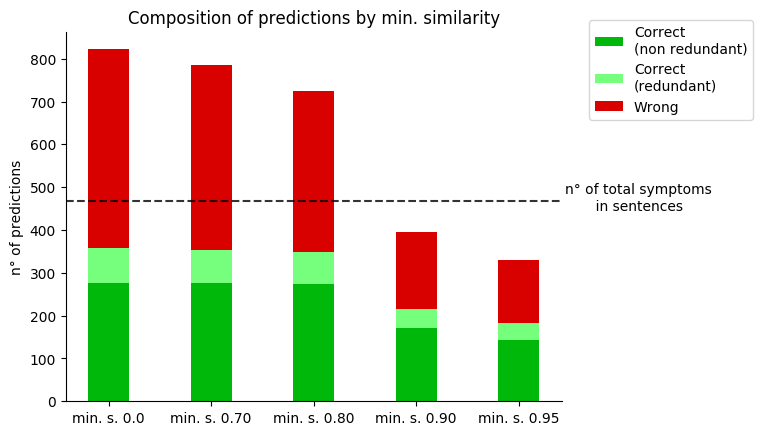
\includegraphics[width=9cm]{graphs/comparison_min_similarity}
    \caption{Comparing the composition of the predictions when different \textit{minimum similarity} levels are used.}
  \end{minipage}
  \hfill
  \begin{minipage}[b]{0.4\textwidth}
    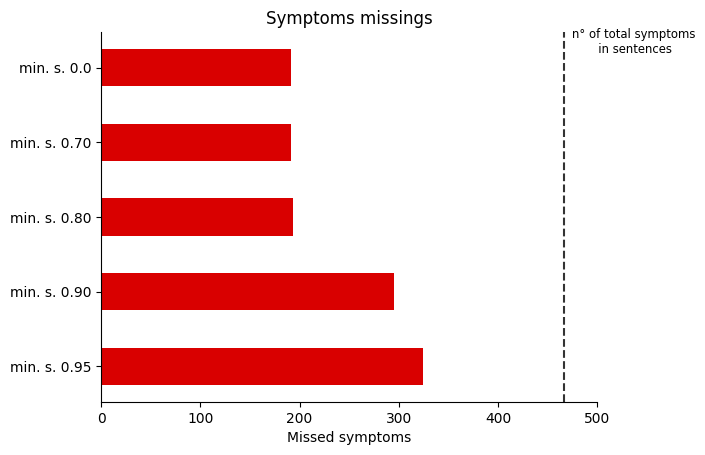
\includegraphics[width=8cm]{graphs/comparison_min_similarity_missings}
    \caption{Comparing the \texttt{missing symptoms} when different \textit{minimum similarity} levels are used.}
  \end{minipage}
\end{figure}

\begin{center}
 \begin{tabular}{| c | c | c | c | c |} 
 \hline
  \thead{\texttt{minimum}\\\texttt{similarity}} & \thead{\texttt{accuracy}} & \thead{\texttt{correct}\\\texttt{predictions}} & \thead{\texttt{medium}\\\texttt{attempts}} & \thead{\texttt{missed}\\\texttt{symptoms}} \\ [0.5ex] 
 \hline\hline
 \texttt{0.00} & 59.1 \% & 43.7 \% & 1.8 & 191 \\ 
 \hline
 \texttt{0.70} & 59.1 \% & 45.1 \% & 1.7 & 191 \\
 \hline
 \texttt{0.80} & 58.7 \% & 48.0 \% & 1.5 & 193 \\
 \hline
 \texttt{0.90} & 36.8 \% & 54.7 \% & 0.8 & 295 \\
 \hline
 \texttt{0.95} & 30.6 \% & 55.3 \% & 0.7 & 324 \\
 \hline
\end{tabular}
\end{center}

%%%%%%%%%%%%%%%%%%%%%%%%%%% discuss data

The objective of this test is to examine if is possible to lower the \texttt{medium attempts} score without penalizing heavily the \texttt{accuracy}. As we can see in the table, it is possible to do it gradually raising the \textit{minimum similarity} level. Apparently, the best performance is gained with a $0.8$ level (the accuracy decreases by 0.4 \% but the medium attempts pass from $1.8$ to $1.5$ and the percentage of correct predictions lifts to 48.0 \%).

The found optimum minimum similarity level is not suitable for each dataset: this meta-parameter could be over-fitted to my examples. However, this test is to interpret as a proof of concept for saying that this is a practicable approach that can lower the number of wrong predictions.

%%%%%%%%%%%%%%%%%%%%%%%%%%%
